\begin{surferIntroPage}{Рекордсмены}{record_chmutovoktic}{Поверхности – рекордсмены}
Поверхность называют \emph{несингулярной} или \emph{гладкой}, если у нее нет заострений или самопересечений (\emph{сингулярностей}), например, шар или тор (см. изображение). Так получается практически в любом случае, когда мы выбираем поверхность произвольным образом.
 \begin{center}
      \vspace{-0.2cm}
      \begin{tabular}{@{}c@{}c@{}c@{\quad}c@{}c@{}c@{}c@{}}
        \begin{tabular}{@{}c@{}}
          гладкие:
        \end{tabular}
        &
        \begin{tabular}{@{}c@{}}
          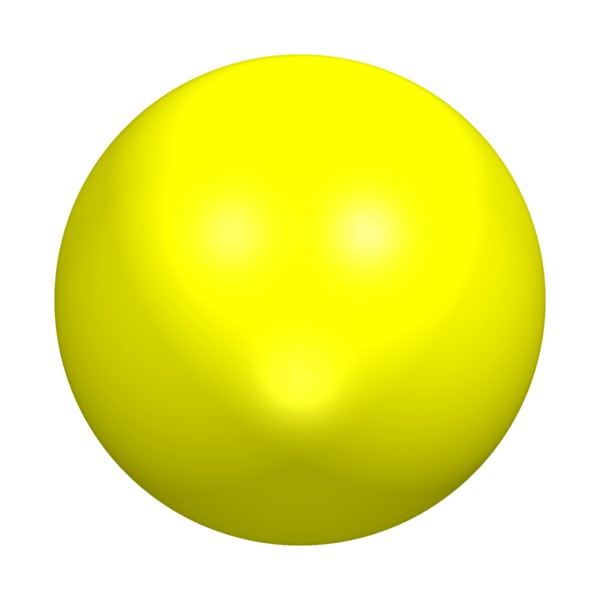
\includegraphics[width=1.1cm]{./../../common/images/kugel}
        \end{tabular}
        &
        \begin{tabular}{@{}c@{}}
          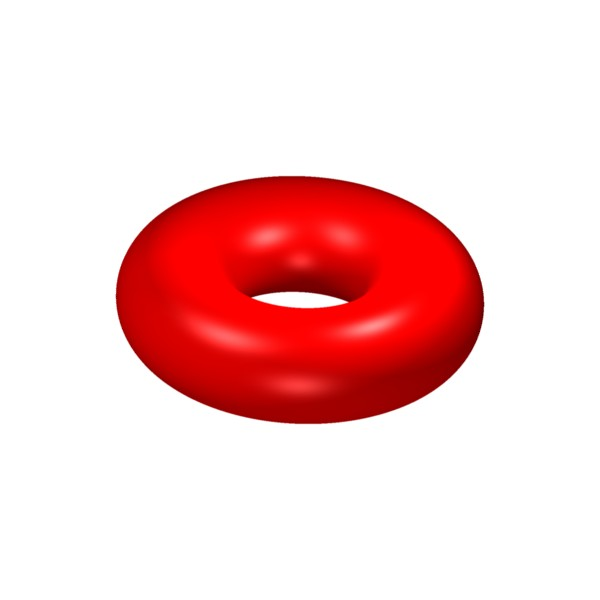
\includegraphics[width=1.1cm]{./../../common/images/torus}
        \end{tabular}
        &
        \begin{tabular}{@{}c@{}}
          со множеством\\
          сингуляностей:
        \end{tabular}
        &
        \begin{tabular}{c@{}@{}}
          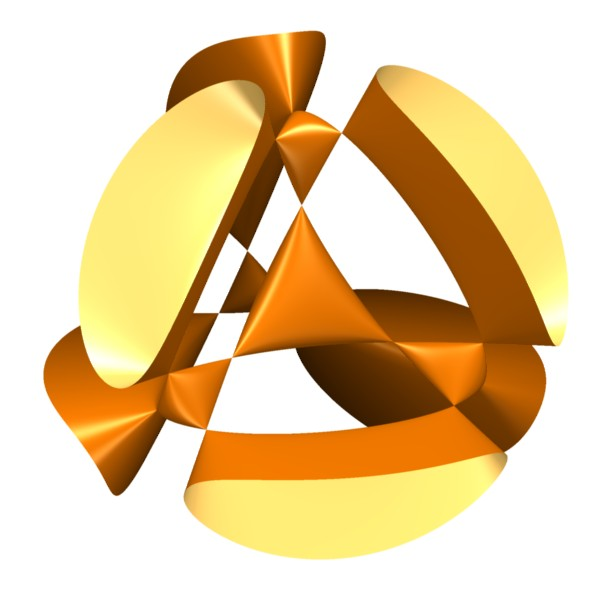
\includegraphics[width=1.1cm]{./../../common/images/kummer}
        \end{tabular}
        &
        \begin{tabular}{c@{}@{}}
          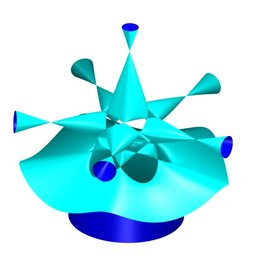
\includegraphics[width=1.1cm]{./../../common/images/togliatti}
        \end{tabular}
        &
        \begin{tabular}{c@{}@{}}
          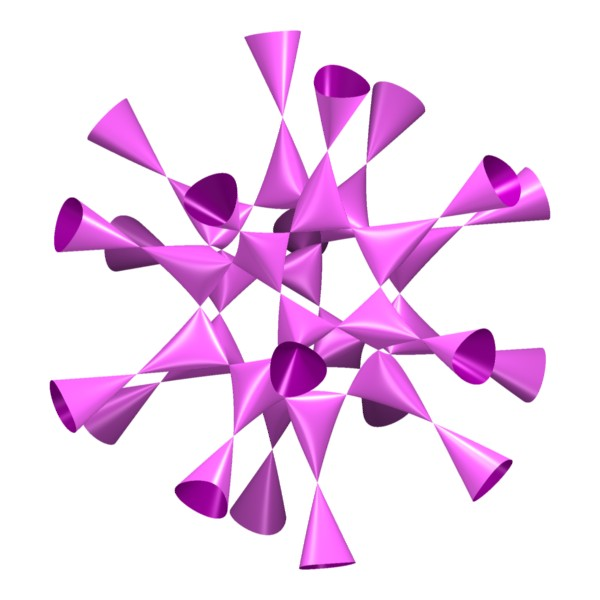
\includegraphics[width=1.1cm]{./../../common/images/barth_sextic}
        \end{tabular}
      \end{tabular}
    \end{center}
    \vspace{-0.2cm}
Лишь особые поверхности обладают точками сингулярности. Это делает сингулярности самыми интересными точками поверхности. Все поверхности в программе SURFER состоят из нулей многочленов. Это значит, что переменные в формулах возводятся лишь в целые положительные степени. Степень старшего монома называют также степенью многочлена.
В математике научный вопрос состоит в том, сколько сингулярностей может иметь поверхность определенной степени. Степень многочлена обозначим через d, а количество сингулярностей через $\mu(d)$. Число $\mu(d)$ очень сложно получить. Для малых показателей степеней, например, $d = 1, 2, 3, 4$ оно известно с $19$ века, для $d = 5$ это число было получено лишь в 1980 г., а для $d = 6$ в 1996 г. Для многочлена седьмой степени максимальное количество сингулярностей неизвестно по сей день. Но есть некоторые исследования, посвящённые этому вопросу. А окончательный ответ на вопрос для любого d лежит ещё в далёком будущем.
Здесь приведены некоторые известные величины:
    \begin{center}
      \begin{tabular}{r|cccccccc|c}
        $d$ & $1$ & $2$ & $3$ & $4$ & $5$ & $6$ & $7$ & $8$ & $d$\\
        \hline
        \hline
        \rule{0pt}{1.2em}$\mu(d)\ge$ & $0$ & $1$ & $4$ & $16$ & $31$ & $65$ &
        $99$ & $168$ & 
        $\approx \frac{5}{12}d^3$\\[0.3em]
        \hline
        \rule{0pt}{1.2em}$\mu(d)\le$ & $0$ & $1$ & $4$ & $16$ & $31$ & $65$ &
        $104$ & $174$ & $\approx \frac{4}{9}d^3$
      \end{tabular}
    \end{center}
\end{surferIntroPage}
